\documentclass[%
 reprint,
%superscriptaddress,
%groupedaddress,
%unsortedaddress,
%runinaddress,
%frontmatterverbose, 
%preprint,
%showpacs,preprintnumbers,
%nofootinbib,
%nobibnotes,
%bibnotes,
 amsmath,amssymb,
 aps,
%pra,
%prb,
%rmp,
%prstab,
%prstper,
%floatfix,
]{revtex4-1}

\usepackage{graphicx}% Include figure files
\usepackage{dcolumn}% Align table columns on decimal point
\usepackage{bm}% bold math
%\usepackage{hyperref}% add hypertext capabilities
%\usepackage[mathlines]{lineno}% Enable numbering of text and display math
%\linenumbers\relax % Commence numbering lines

%\usepackage[showframe,%Uncomment any one of the following lines to test 
%%scale=0.7, marginratio={1:1, 2:3}, ignoreall,% default settings
%%text={7in,10in},centering,
%%margin=1.5in,
%%total={6.5in,8.75in}, top=1.2in, left=0.9in, includefoot,
%%height=10in,a5paper,hmargin={3cm,0.8in},
%]{geometry}

\usepackage{cmap} % Поиск в PDF
\usepackage[T2A]{fontenc} % Кодировка
\usepackage[utf8]{inputenc} % Кодировка исходного текста
\usepackage[english, russian]{babel} % Локализация и переносы
\frenchspacing % Более тонкая настройка пробелов 
\usepackage{multirow}
\usepackage[warn]{mathtext}
\usepackage{amssymb}
\usepackage{ dsfont }

% Переопределение англоязычного начертания каппа, фи и эпсилон, 
% а также знаков сравнения
\renewcommand{\epsilon}{\ensuremath{\varepsilon}}
\renewcommand{\phi}{\ensuremath{\varphi}} 
\renewcommand{\kappa}{\ensuremath{\varkappa}}
\renewcommand{\le}{\ensuremath{\leslant}}
\renewcommand{\leq}{\ensuremath{\leqslant}}
\renewcommand{\ge}{\ensuremath{\geslant}}
\renewcommand{\geq}{\ensuremath{\geqslant}}
\renewcommand{\emptyset}{\ensuremath{\varnothing}}

\usepackage{textcomp} 
\usepackage{indentfirst} % Красная строка
\usepackage{amsmath} % Текст в формулах
\usepackage{graphicx} % Графика
\DeclareGraphicsExtensions{.pdf,.png,.jpg}
\usepackage{pgfplots}
\pgfplotsset{compat=1.13}

%\usepackage{times}

\begin{document}

\title{Сдвиг фаз в цепи переменного тока}
\thanks{3.2.1}

\author{Иван Едигарьев,}
\affiliation{
 Московский Физико-Технический Институт\\
 Факультет Общей и Прикладной Физики, 526т\\
}
%\date{\today}

\begin{abstract}
Цель работы: изучить влияние активного сопротивления, индуктивности и ёмкости на сдвиг фаз между током и напряжением в цепи переменного тока.

В работе используются: генератор звуковой частоты (ЗГ), двухканальный осциллограф (ЭО), магазин ёмкостей, магазин сопротивлений, катушка индуктивности, резисторы, мост переменного тока.

\end{abstract}

\pacs{Valid PACS appear here}% PACS, the Physics and Astronomy
                             % Classification Scheme.
%\keywords{Suggested keywords}%Use showkeys class option if keyword
                              %display desired
\maketitle

%\tableofcontent

\section{\label{sec:level1}Теоретическая справка}

Удобным, хотя и не очень точным прибором для измерения фазовых соотношений служит электронный осциллограф. Пусть нужно измерить сдвиг фаз между двумя напряжениями $U_1$ и $U_2$. Подадим эти напряжения на горизонтальную и вертикальную развёртки осциллографа. Смещение луча по горизонтали и вертикали определяется выражениями:
$$ x = x_0 \cos{\Omega t} ~~~~~ y = y_0 \cos{(\Omega t + \alpha)}$$
где $\alpha$ — сдвиг фаз между напряжениями $U_1$ и $U_2$, а $x_0$ и $y_0$ — амплитуды напряжений, умноженные на коэффициенты усиления соответствующих каналов осциллографа. Исключив время, после несложных преобразований найдём:

$$ \left( \frac{x}{x_0} \right)^2 + \left( \frac{y}{y_0} \right)^2 + \frac{2 x y}{x_0 y_0} \cos{\alpha} = \sin^2{\alpha}$$

Полученное выражение определяет эллипс, описываемый электронным лучом на экране осциллографа (рис. 1). Ориентация эллипса зависит как от искомого угла $\alpha$, так и от усиления каналов осциллографа. Для расчёта сдвига фаз можно измерить отрезки $2 y_{x=0}$ и $2y_0$ (или $2 x_{y=0}$ и $2x_0$, на рисунке не указанные) и, подставляя эти значения в уравнение эллипса, найти

$$\alpha = \pm \arcsin{\left( \frac{y_{x=0}}{y_0}\right)}$$
Для правильного измерения отрезка $2y_{x=0}$ важно, чтобы центр эллипса лежал на оси y.

На практике часто используются устройства, позволяющие в широких пределах изменять фазу напряжения (0 < $\psi$ < $\pi$). Такие устройства называются фазовращателями. Схема простого фазовращателя приведена на рис. 2. Она включает в себя два одинаковых резистора $R_1$, ёмкость $C$ и переменное сопротивление $R$.

Используя метод комплексных амплитуд, найдём зависимость сдвига фаз между входным напряжением $U_{\text{вх}}$ = $U_0 \cos{\Omega t}$ и выходным $U_{\text{вых}}$ от соотношения между импедансами сопротивления $R$ и ёмкости $C$. Для этого выразим выходное напряжение $U_{\text{вых}}$ через $U_{\text{вх}}$, параметры контура и частоту внешнего источника $\Omega$: $U_{34} = f(U_{12},~R,~C,~\Omega)$.

Обозначим комплексную амплитуду входного напряжения через $\widehat{U}_0$. Тогда напряжение между точками 1 и 3 в силу равенства сопротивлений $R_1$
$$ \widehat{U}_{13} = \frac{\widehat{U}_0}{2}. $$
Если фазу напряжения $\widehat{U}_{\text{вх}}$ положить равной нулю, то $\widehat{U}_0$ будет действительной величиной: $\widehat{U}_0 = U_0$. Приняв напряжение в точке 1 равным нулю, получим амплитуду напряжения в точке 3:
$$ \widehat{U}_{03} = \frac{U_0}{2}. $$
Рассчитаем $\widehat{U}_{04}$ — амплитуду напряжения в точке 4. Импеданс $Z$ последовательно соединённых сопротивления $R$ и ёмкости $C$ равен:
$$ Z = R - \frac{i}{\Omega C}. $$
Для комплексной амплитуды тока $\widehat{I}_0$, проходящего через $R$ и $C$, имеем
$$ \widehat{I}_0 = \frac{U_0}{Z} = \frac{U_0}{R - i/(\Omega C)},$$
а для комплексной амплитуды напряжения в точке 4
$$ \widehat{U}_{04} = \widehat{I}_0 R = U_0 \frac{R}{R - i/(\Omega C)}.$$
Выходное напряжение $\widehat{U}_{\text{вых}}$ равно разности напряжений в точках 3 и 4:
$$\widehat{U}_{\text{вых}} = \widehat{U}_{04} - \widehat{U}_{03} = \widehat{U}_{04} - U_0 /2 = \frac{U_0}{2} \frac{R + i/(\Omega C)}{R - i/(\Omega C)}.$$

В числитель и знаменатель последнего выражения входят комплексносопряжённые величины, модули которых одинаковы, поэтому величина выходного напряжения не меняется при изменении $R$. Модуль $U_{\text{вых}}$ всегда равен $U_0 /2$ — половине $U_{\text{вх}}$. Сдвиг фаз между входным и выходным напряжениями равен $2 \arctg[1/(\Omega R C)]$ и меняется от $\pi$ (при $R \rightarrow 0$) до 0 (при $R \rightarrow \infty$).

\section{\label{sec:level1}Экспериментальная установка}

Схема для исследования сдвига фаз между током и напряжением в цепи переменного тока представлена на рис. 3. Эталонная катушка $L$, магазин ёмкостей $C$ и магазин сопротивлений $R$ соединены последовательно и через дополнительное сопротивление $r$ подключены к источнику синусоидального напряжения — звуковому генератору ГЗ-109.

Сигнал, пропорциональный току, снимается с сопротивления $r$, пропорциональный напряжению — с генератора. Оба сигнала подаются на универсальный осциллограф С1-83. Этот осциллограф имеет два канала вертикального отклонения, что позволяет одновременно наблюдать на экране два сигнала. В нашей работе это две синусоиды, смещённые друг относительно друга в зависимости от сдвига фаз между током и напряжением в цепи. На рис. 3 синусоиды на экране ЭО сдвинуты по фазе на $\pi /2$.

Схема фазовращателя, изображённая на рис. 4, содержит два одинаковых резистора $R_1$, смонтированных на отдельной плате, магазин сопротивлений $R$ и магазин ёмкостей $C$.

\section{\label{sec:level1}Задание}

Данное описание даётся ссылкой на [1]. Пункты задания из [1] сохраняют свою нумерацию и в этой работе.

\section{\label{sec:level1}Данные}

Для $RC$-цепи построим по измеренным данным график зависимости $\psi = f(R_{\Sigma})$ (График 1) и $\tg(\psi) = f(1/(\Omega C R_{\Sigma}))$ (График 2). Второй график выполним в логарифмической шкале ради упрощения анализа зависимости\\
\\
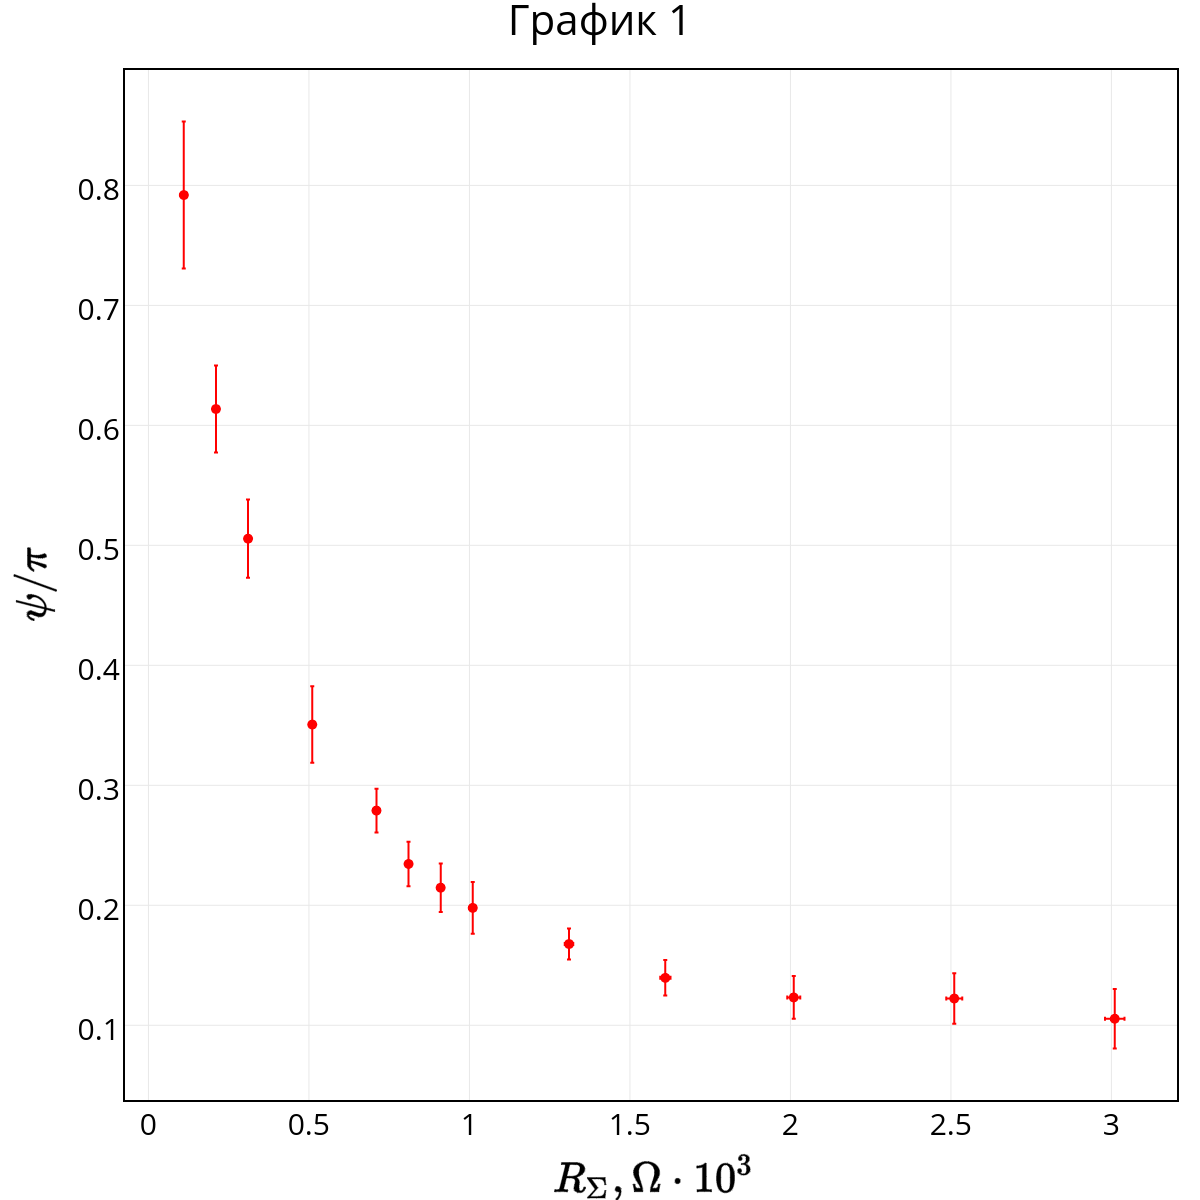
\includegraphics[scale=0.19]{my_plot1.png}\\
\\
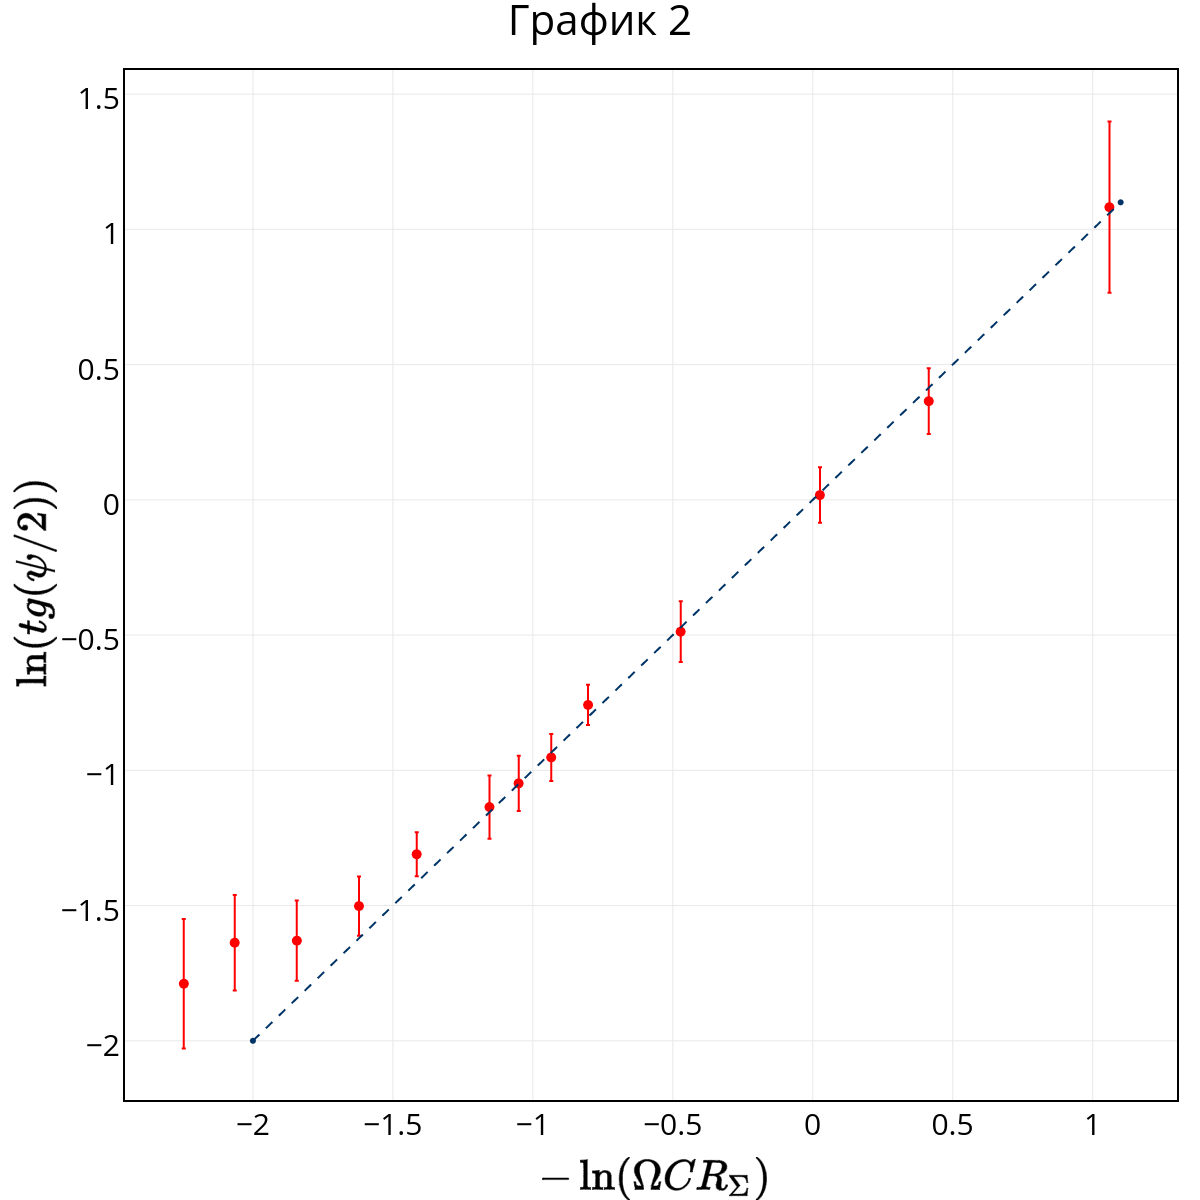
\includegraphics[scale=0.19]{my_plot2.png}
\\

На втором графике дополнительно изображена теоретическая зависимость. По графику $\tg(\psi) = f(1/(\Omega C R_{\Sigma}))$ можно сказать, что теоретическая закономерность верна в рамках систематической ошибки. А также, что реактивное сопротивление цепи совпадает с сопротивлением, соответствующим сдвигу фаз $\psi = \pi/2$, равным $X_1(\Omega) = \Omega L = 314,1~\Omega$.

Проделаем аналогичную процедуру теперь для $RL$-цепи. Построим графики, соответствующие новым зависимостям.\\
\\
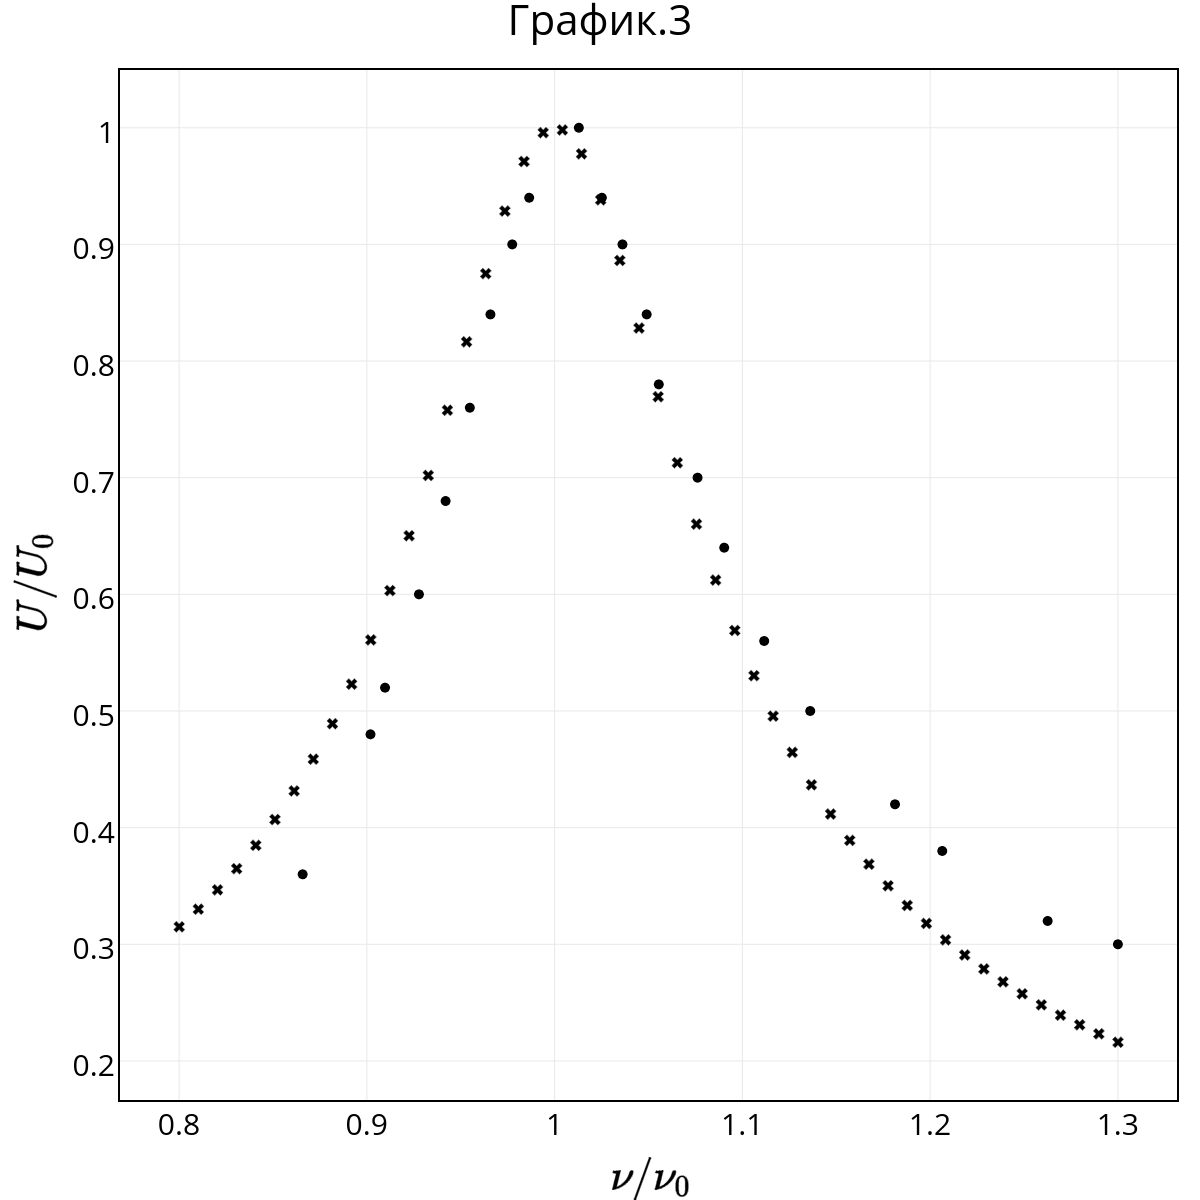
\includegraphics[scale=0.19]{my_plot3.png}\\
\\
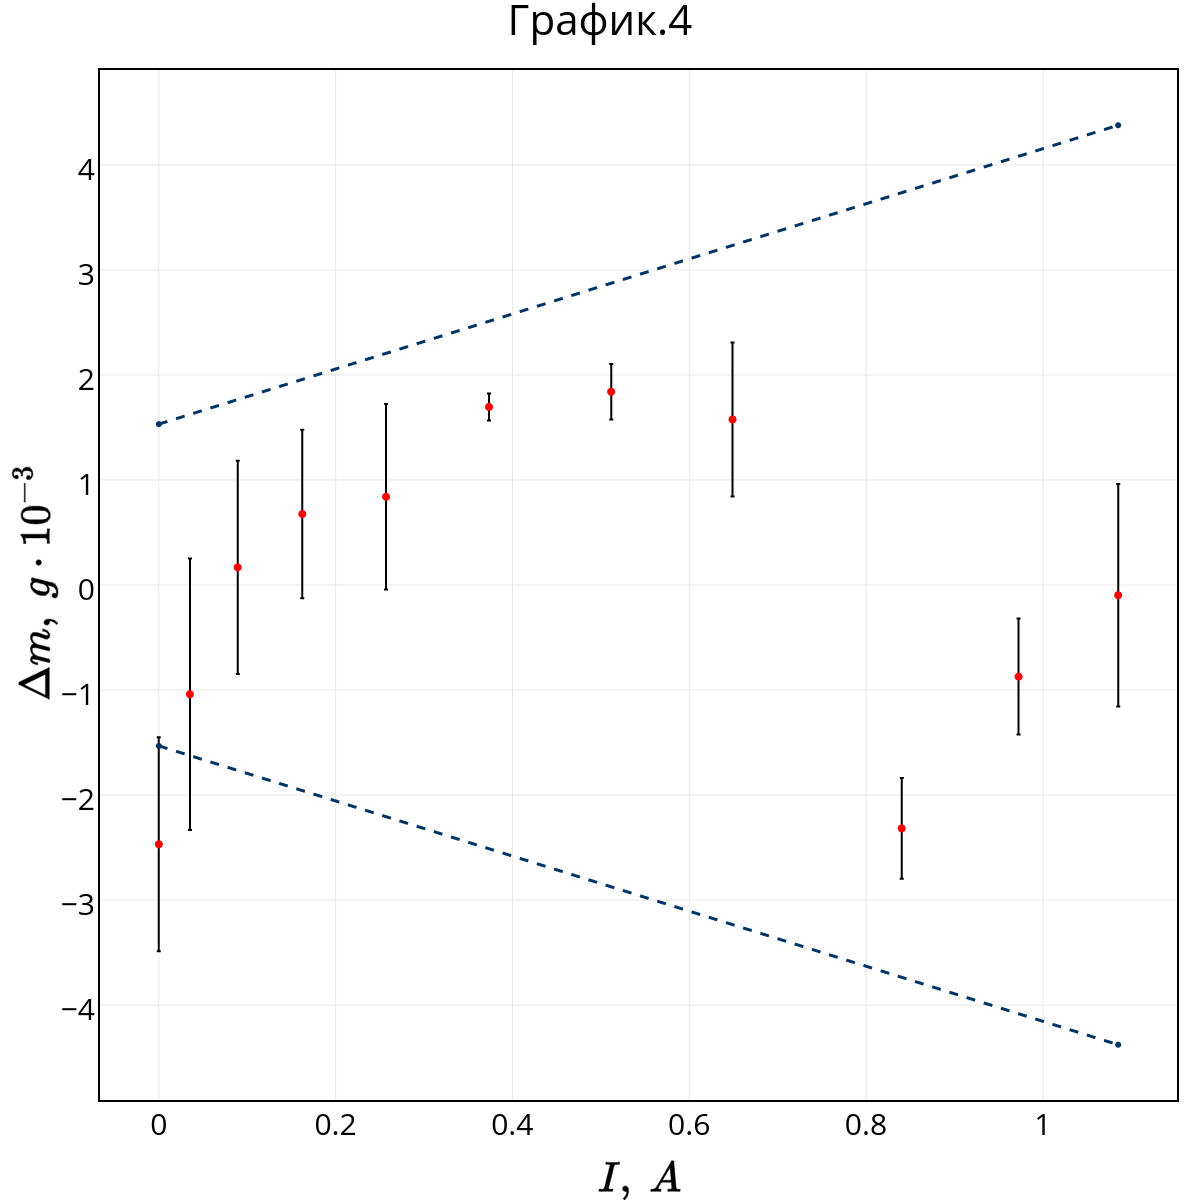
\includegraphics[scale=0.19]{my_plot4.png}

Легко видеть, что все измеренные точки согласуются с теоретической зависимостью с точностью до 95\% доверительного интервала, и все, кроме одной, с точностью до 66\% доверительного интервала. Аналогично реактивное сопротивление согласуется с теоретическим, что можно видеть из второго и первого графика. $X_2(\Omega) = 1/(\Omega C) = 318,3~\Omega$

Теперь построим резонансные кривые $|\psi| = f(\nu/\nu_0)$, соответствующие $R=0$ и $100~\Omega$. \\
\\
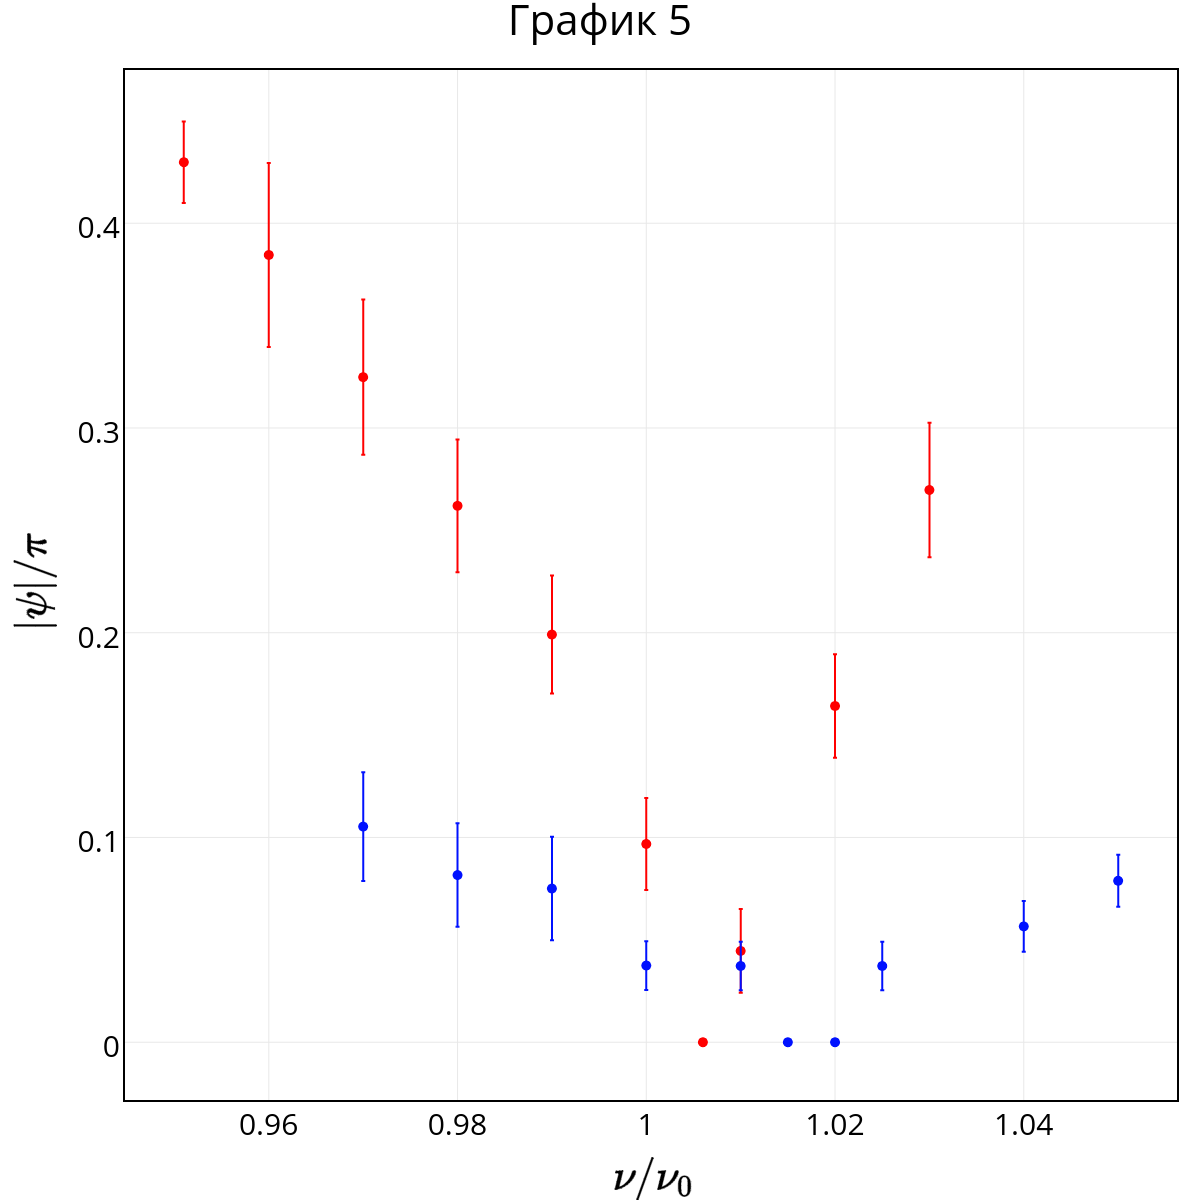
\includegraphics[scale=0.19]{my_plot5.png}

В данной работе предлагает воспользоваться методом измерения ширины резонансной кривой при сдвиге фаз $\psi = \pi/4$ для вычисления добротности контура. Данный способ является в некоторой степени эмпирическим и не претендует на абсолютную точность. Поэтому воспользуемся другим методом, а именно будем делать двухпараметрический фит, под зависимость:
$$ \cos{\psi} = \left(1 + Q^2 \left(\frac{2\Delta \nu}{\nu_0}\right)^2\right)^{-1/2},$$

где параметрами модели будут $\nu_0$ и $Q$ ($\Delta \nu = \nu - \nu_0$).

В итоге. Для $R=0$:\\
\\
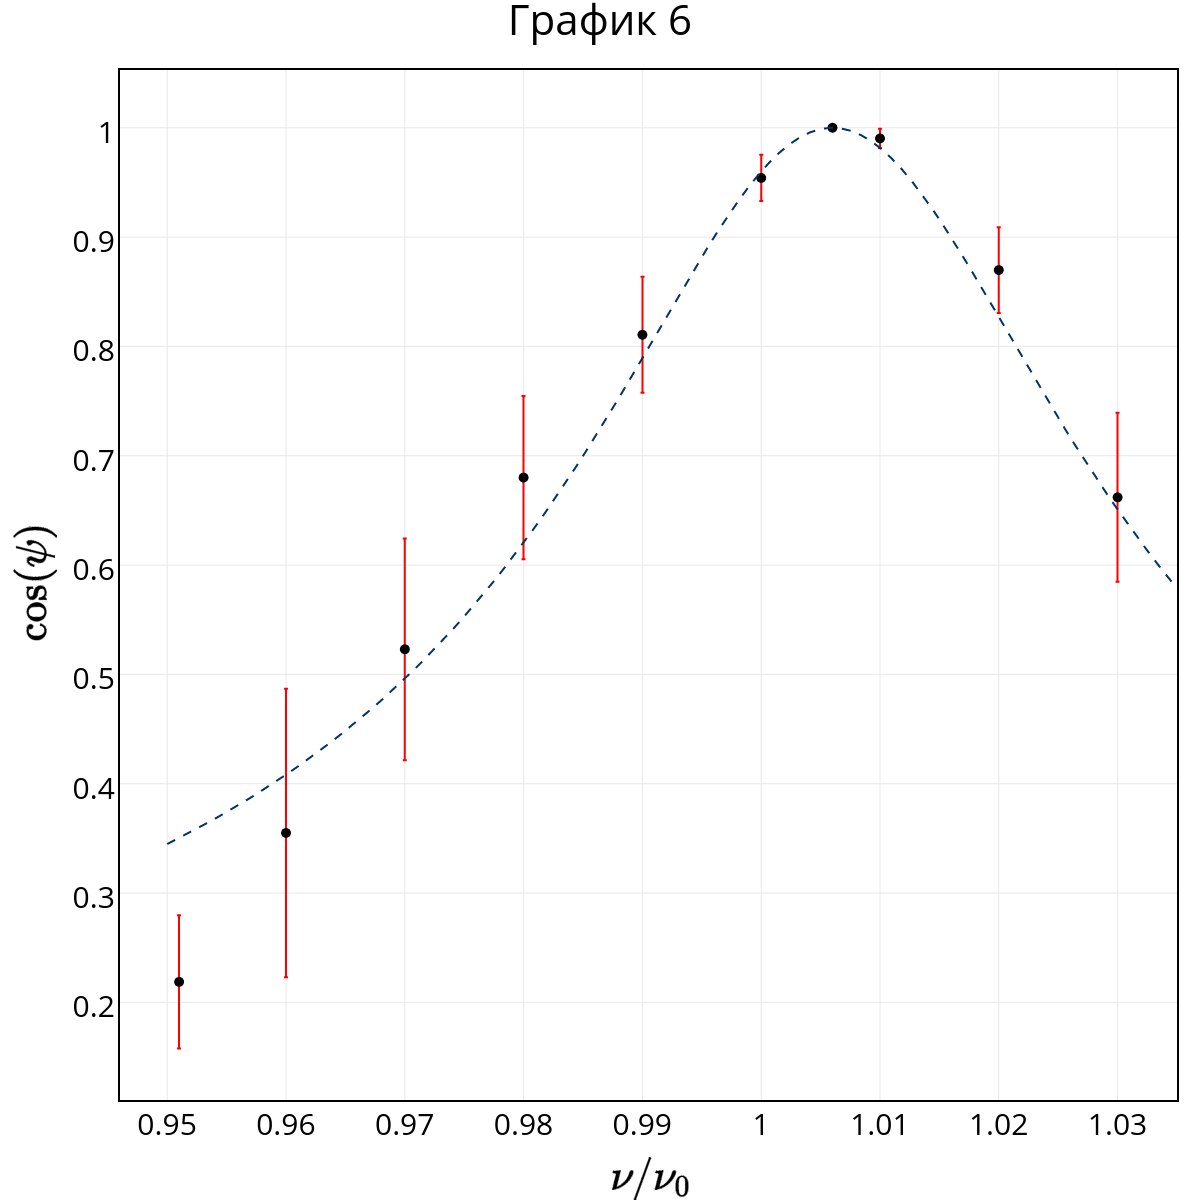
\includegraphics[scale=0.19]{my_plot6.png}
$$\boxed{Q^{\text{fit}} = 25 \pm 2^{\text{stat}},~~~\nu_0^{\text{fit}} = (1006 \pm 2^{\text{stat}})~Hz}$$

Для $R=100~\Omega$:\\
\\
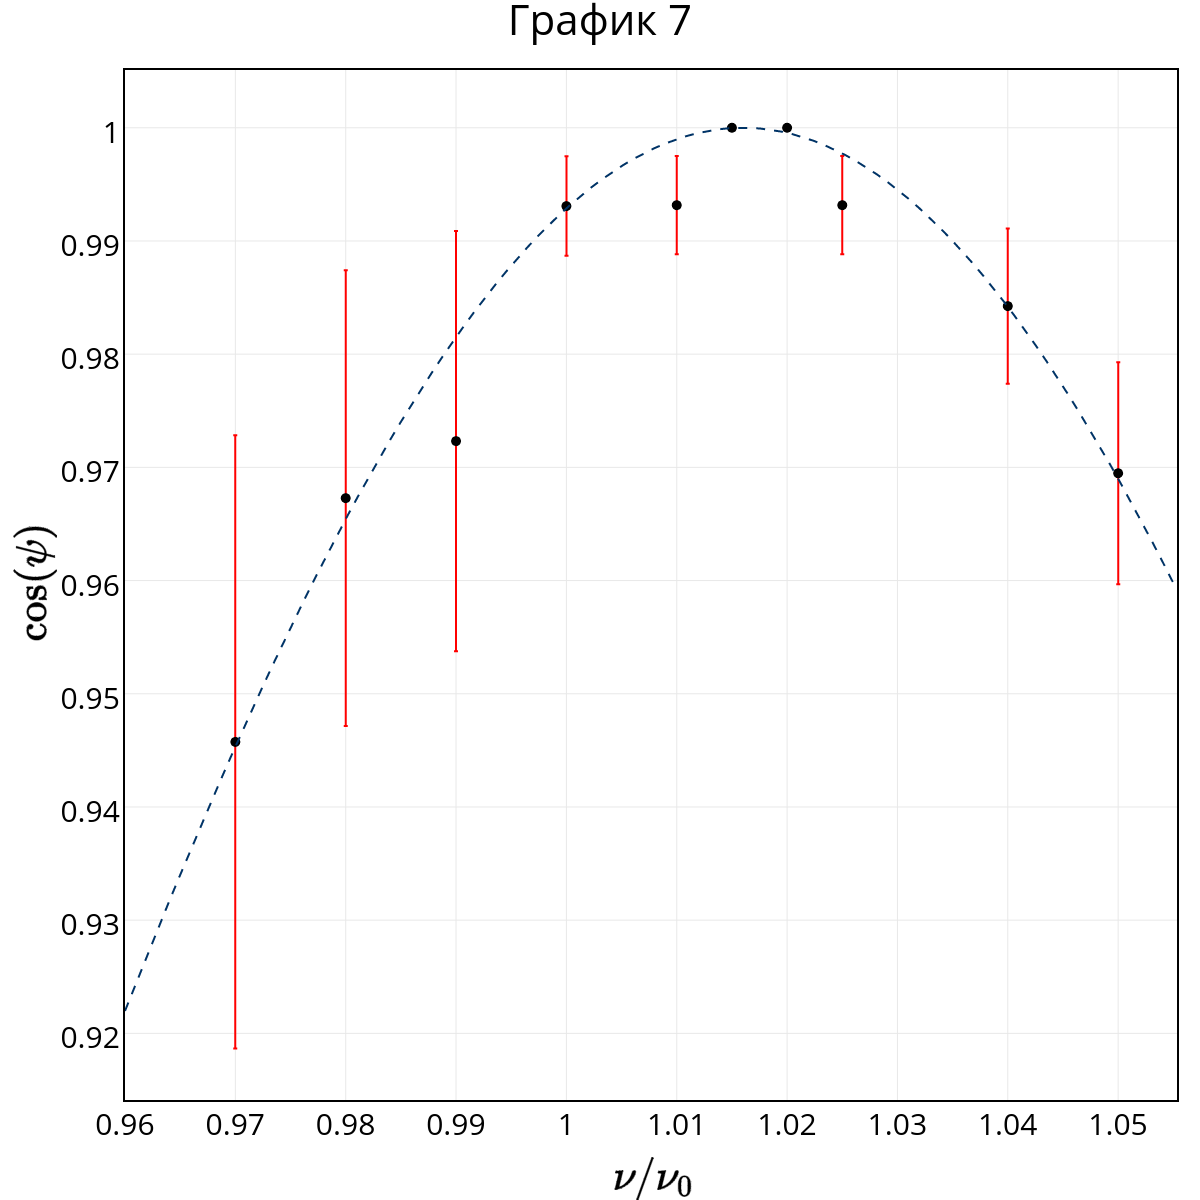
\includegraphics[scale=0.19]{my_plot7.png}
$$\boxed{Q^{\text{fit}} = 4 \pm 1^{\text{stat}},~~~\nu_0^{\text{fit}} = (1016 \pm 1^{\text{stat}})~Hz}$$

Во втором случае при $R=100 \Omega$ во время эксперимента было проведено недостаточно измерений для определения добротности электрической цепи первым, предложенным в методической рекомендации, способом.

Рассчитаем добротность для двух конфигураций цепи через параметры контура:
$$\text{для~}R=0~\Omega:~Q^{\text{theory}} = 30.7 \pm 0.3^{\text{syst}}$$ $$\text{для~}R=100~\Omega:~Q^{\text{theory}} = 2.9 \pm 0.3^{\text{syst}}$$

Построим векторную диаграмму для фазовращателя и рассчитаем сопротивление магазина $R_{\text{M}}$, при котором сдвиг фаз между входным и выходным напряжениями равен $\pi/2$. Данные вычисления приведены в Приложении 1.

Сведём результаты в итоговую таблицу:\\
\\
\\
\\
\\
\\
\\
\\
\\
\section{\label{sec:level1}Ссылки}
[1] - Лабораторный практикум по общей физике. Электричество и магнетизм. МФТИ, 2007. ISBN 5-7417-0204-x (T. 2)
\end{document}